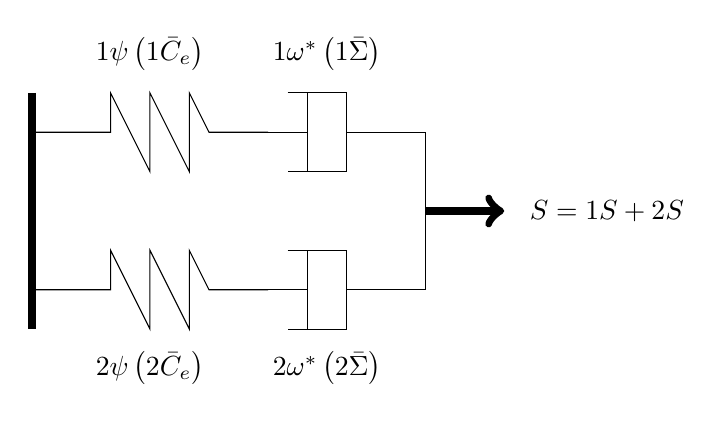
\begin{tikzpicture}
    % Spring 1
    \draw[-] (0,0) -- (1,0) -- (1,0.5) -- (1.5,-0.5) -- (1.5,0.5) -- (2,-0.5) -- (2,0.5) -- (2.25,0) -- (3,0);
    % dashpot 1
    \draw[-] (3,0) -- (3.5,0) -- (3.5,0.5) -- (3.5,-0.5);
    \draw[-] (3.25,0.5) -- (4,0.5) -- (4,-0.5) -- (3.25,-0.5);
    \draw[-] (4,0) -- (5,0);
    % Spring 2
    \draw[-] (0,0-2) -- (1,0-2) -- (1,0.5-2) -- (1.5,-0.5-2) -- (1.5,0.5-2) -- (2,-0.5-2) -- (2,0.5-2) -- (2.25,0-2) -- (3,0-2);
    % dashpot 2
    \draw[-] (3,0-2) -- (3.5,0-2) -- (3.5,0.5-2) -- (3.5,-0.5-2);
    \draw[-] (3.25,0.5-2) -- (4,0.5-2) -- (4,-0.5-2) -- (3.25,-0.5-2);
    \draw[-] (4,0-2) -- (5,0-2);
    % left boundary
    \draw[-,line width = 3pt] (0,0.5) -- (0,-2.5);
    % right boundary
    \draw[-] (5,0) -- (5,0-2);
    \draw[->,line width = 3pt] (5,-1) -- (6.0,-1);
    % description
    \node (psi1) [] at (1.5,1.0) {$\prescript{1}{}{}\psi\left(\prescript{1}{}{}\bar{\bm{C}}_e\right)$};
    \node (psi2) [] at (1.5,-3.0) {$\prescript{2}{}{}\psi\left(\prescript{2}{}{}\bar{\bm{C}}_e\right)$};
    \node (w1) [] at (3.75,1.0) {$\prescript{1}{}{}\omega^*\left(\prescript{1}{}{}\bar{\bm{\Sigma}}\right)$};
    \node (w2) [] at (3.75,-3.0) {$\prescript{2}{}{}\omega^*\left(\prescript{2}{}{}\bar{\bm{\Sigma}}\right)$};
    \node (S) [anchor=west] at (6.2,-1) {$\bm{S} = \prescript{1}{}{}\bm{S} + \prescript{2}{}{}\bm{S}$};
\end{tikzpicture}